
%(BEGIN_QUESTION)
% Copyright 2007, Tony R. Kuphaldt, released under the Creative Commons Attribution License (v 1.0)
% This means you may do almost anything with this work of mine, so long as you give me proper credit

A graphical aid in understanding transistor amplifier circuits is something called a {\it load line}.  Here is a simple transistor amplifier with a corresponding load line superimposed on the characteristic curve graph:

$$\includegraphics[width=15.5cm]{i02477x01.eps}$$

Explain how this ``load line'' is calculated and plotted, and also what it means for this amplifier circuit.

\vskip 10pt

Power sources and power conditioner circuits for intrinsically safe instrument loops also have ``load line'' characteristics because they must limit the amount of energy available to the field instrument, and they can only do so by limiting voltage and/or current.  Passive power sources exhibit linear load characteristics just like the transistor amplifier shown above.  For example, a passive (``entity model'') FOUNDATION Fieldbus power source has the following voltage/current characteristics, and may be modeled as a simple Th\'evenin circuit (voltage source and series resistance):

$$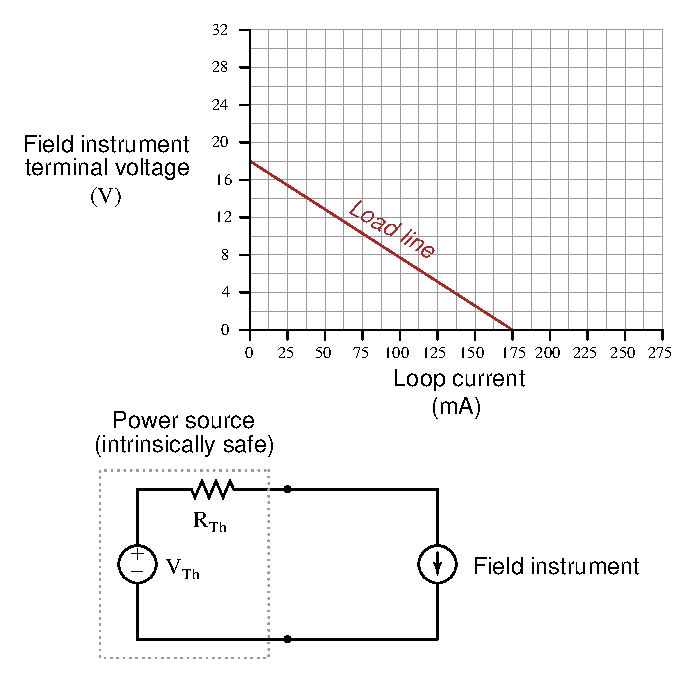
\includegraphics[width=15.5cm]{i02477x02.eps}$$

Calculate the necessary $V_{Th}$ and $R_{Th}$ values to generate the load line shown for this passive circuit.

\vskip 10pt

\filbreak

``Active'' power sources are more complex, but they allow slightly greater levels of power to be delivered to the field instrument without exceeding the limits of voltage and current necessary to meet intrinsic safety standards.  Shown here is a non-linear ``load line'' and (simplified) circuit for an active, intrinsically safe power source:

$$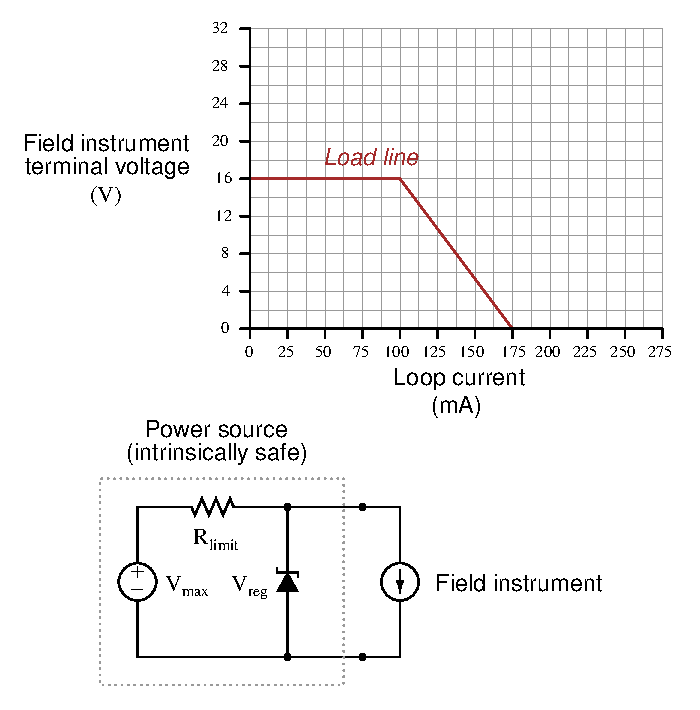
\includegraphics[width=15.5cm]{i02477x03.eps}$$

Calculate the necessary $V_{max}$, $V_{reg}$ ($V_{zener}$), and $R_{limit}$ values to generate the load line shown for this passive circuit.  Note: the zener diode shown in this circuit is actually a complete voltage regulator circuit in an actual active power source.  However, for the purposes of this analysis, a simple zener diode will suffice.

\underbar{file i02477}
%(END_QUESTION)





%(BEGIN_ANSWER)

\noindent
{\bf Passive power source:}

$V_{Th}$ = 18 volts \hskip 50pt $R_{Th}$ = 102.9 $\Omega$

\vskip 10pt

\noindent
{\bf Active power source:}

$V_{max}$ = 37.33 volts \hskip 50pt $V_{reg}$ = 16 volts \hskip 50pt $R_{limit}$ = 213.33 $\Omega$

\vskip 10pt

Challenge question: calculate the maximum possible power delivered to the field instrument for both of these power sources, and explain {\it how} you calculated these values.

%(END_ANSWER)





%(BEGIN_NOTES)

The active power source can deliver a maximum of 1.6 W to the field instrument (power calculated at the corner of the non-linear graph: 16 V $\times$ 100 mA).

The passive power source achieves maximum power output to the field device when the field device's equivalent resistance is equal to $R_{Th}$, as predicted by the Maximum Power Transfer theorem.  This places both the voltage and current at half their maximum values.  Thus, the passive source can deliver a maximum of 0.7875 W to the field instrument (9 V $\times$ 87.5 mA).

%INDEX% Electronics review: transistor load lines
%INDEX% Safety, intrinsic: linear versus trapezoidal power supply characteristic

%(END_NOTES)


